\documentclass[12pt,letterpaper]{article}  
%%%%%%%%INSTALACION DE PAQUETES%%%%%%%%%%%%%%%%%%%%%%%%%%%
\input{config}

\lhead{Circuitos electrónicos 1}
	\chead{}
	\rhead{Osciladores senoidales}
	%\lfoot{Facultad de Ingeniería}
	\cfoot{\thepage\ de \pageref{LastPage}}
	%\rfoot{Universidad Nacional de Mar del Plata}

% Comandos especiales
\newcommand{\EIE}{\textsc{Facultad \Lightning~ Ingeniería}}
%---------------INICIO DE DOCUMENTO--------------
\begin{document}

% portada
\begin{titlepage}
                




\centering
\hspace{10pt}

\begin{figure}[h]
\centering
\fbox{\includegraphics[width=0.8\linewidth]{images/math.jpg}}
\label{1.0}
\end{figure}


{\scshape\Huge  \par}
{\scshape\Huge Matemática \par}
\vspace{1cm}

{\Large Autor: \par}
{\Large Vazquez, Leonardo David \par}
\vspace{1cm}

{\Large Contacto: \par}
{\Large vazquezleonardodavid@outlook.com \par}
\vspace{1cm}

\end{titlepage}

%\maketitle
%\thispagestyle{empty} 
%\maketitle

{
  \hypersetup{linkcolor=black}
  \tableofcontents
}

% RESUMEN
\section*{Resumen}

\setlength{\parindent}{12pt}
En el presente trabajo, se propone realizar un análisis teórico de distintos circuitos que funcionan como osciladores senoidales.
\bigskip

%OSCILADORES SENOIDALES
\newpage
\section{Osciladores senoidales}
   \subsection{Fundamentos teóricos}
      En los sistemas electrónicos surge con frecuencia la necesidad de contar con señales periódicas como por ejemplo señales senoidales. En particular, el método que se utiliza es el del concepto de realimentación y consiste en un amplificador y una red selectiva en frecuencia R-C o L-C. 

En este punto se estudian los principios básicos de los osciladores lineales, el cual se tiene que emplear alguna forma de no linealidad para obtener el control de la amplitud de la onda de salida. De hecho todos los osciladores son, estrictamente hablando, circuitos no lineales.
Para poder utilizar las herramientas de análisis y diseño de sistemas lineales se procede en dos pasos: primero se considera al sistema idealmente lineal, utilizando los criterios circuitales y de realimentación conocidos; y luego se hace uso de mecanismos no lineal para controlar la amplitud. 

En la figura \ref{1.0} se muestra un sistema realimentado. Considerando el límite de estabilidad: $1 + T(s) = 1 + a(s)f(s) = 0$.

%%paquete de tikz
\tikzstyle{startstop} = [rectangle, rounded corners, minimum width=3cm, minimum height=1cm,text centered, draw=black, fill=red!30]
\tikzstyle{io} = [trapezium, trapezium left angle=70, trapezium right angle=110, minimum width=3cm, minimum height=1cm, text centered, draw=black, fill=blue!30]
\tikzstyle{process} = [rectangle, minimum width=3cm, minimum height=1cm, text centered, draw=black, fill=orange!30]
\tikzstyle{decision} = [diamond, minimum width=3cm, minimum height=1cm, text centered, draw=black, fill=green!30]
\tikzstyle{arrow} = [thick,->,>=stealth]
\tikzstyle{line} = [thick,-,>=stealth]


\tikzstyle{beta} = [diamond, minimum width=3cm, minimum height=1cm, text centered, draw=black, fill=green!50] 
\tikzstyle{amp} = [rectangle, minimum width=3cm, minimum height=1cm, text centered, draw=black, fill=orange!50]
%%%%%%%%%%%%%%%%%%%%%%%
\begin{figure}[H]
    \centering
     \begin{tikzpicture}[node distance=2cm]
                       \node (amp) [amp] {$a(s)$};
                       \node (beta) [beta, below of=amp] {$\beta (s)$};
                       \draw [arrow] (-3,0) -- (amp);
                       \draw [arrow]  (amp) -- (3,0);
                       \draw [arrow] (beta) -- (-3,-2);
                       \draw [arrow] (3,-2) -- (beta);
                       \draw [thick] (3,-2) -- (3,0) ;
                       \draw [thick] (-3,0) -- (-3,-2);
    \end{tikzpicture}
\caption{Esquema de un oscilador senoidal.$a(s)$: amplificador. $\beta (s)$ = red selectiva de frecuencia.}
\label{1.0}
\end{figure}




\subsubsection{Criterio de oscilación}

Si a una frecuencia angular específica $w_o$ la ganancia de lazo $\mid a(w_o)\cdot \beta(w_o)\mid =1$, el sistema sería un oscilador, es decir, tendría una salida finita sin excitación en su entrada. Para que el sistema oscile senoidalmente a la frecuencia $w_o$ la condición antedicha sólo debe cumplirse a una tal frecuencia. Esto se conoce como criterio de oscilación de Barkhausen.

El criterio de Barkhausen puede desdoblarse en:

\begin{equation}
\label{eq:1_1}
\mid a(w_o)\cdot \beta (w_o)\mid =1  
\end{equation}

\begin{equation}
\label{eq:1_2}
\Phi \{a(w_o)\cdot \beta (w_o)\} = 0  
\end{equation}

La expresión \ref{eq:1_1} es la denominada condición de amplitud. En la práctica, la red $\beta$ es una red selectiva en frecuencia, siendo $w_o$ su frecuencia central de mínima atenuación. A dicha frecuencia la amplificación $a(w_o)$ sería igual a la inversa de la atenuación de la red selectiva en frecuencia $\beta (w_o)$, de modo que la ganancia de lazo total sea unitaria. En cambio, la expresión $\ref{eq:1_2}$ es la condición de fase, que establece que el desfasaje de la ganancia de lazo debe ser nulo a la frecuencia $w_o$.

\subsubsection{Control no lineal de amplitud}

El criterio de oscilación de Barkhausen garantiza oscilaciones senoidales en un sentido matemático. Si por medio de ajustes se lograra que el sistema cumpla exactamente la condición de amplitud, es sabido que esta situación sería imposible de mantenerla en el tiempo, ya que variaciones inevitables de los parámetros (por ejemplo por temperatura) harían que los polos imaginarios puros se desplazaran a uno u otro lado en el plano $S$. Si los polos se desplazaran hacia la izquierda del eje imaginario (zona estable) las oscilaciones cesarían. Por el contrario, si los polos se movieran hacia el semiplano derecho, la amplitud de las oscilaciones tendería a aumentar siendo limitadas por la saturación de los dispositivos activos, generando señales oscilantes con alto grado de distorsión. Es sabido, además, que la amplitud de la señal de salida de un sistema con polos en el eje imaginario depende en forma teórica de las condiciones iniciales. Estos dos efectos, la variación de los parámetros y la dependencia de la amplitud de salida de las condiciones iniciales, hacen necesario un mecanismo de control no lineal de la ganancia del sistema.

Básicamente el mecanismo de control debe cumplir con lo siguiente: 
\begin{itemize}
    \item En primera instancia se debe diseñar el sistema para que los polos se encuentren en la mitad derecha del plano $S$, con la precaución de que estén cercanos al eje imaginario $j$. Esta condición se obtiene modificando el criterio de Barkhausen de modo que se cumpla la condición de fase y que se cumpla en exceso la condición de amplitud:  $\mid a(w_o)\cdot \beta(w_o)\mid > 1$, de
    esta manera aseguramos que los polos iniciales estén en el semiplano derecho. Para que no haya excesiva distorsión no lineal en la señal de salida, la condición de amplitud debe diseñarse
    para que se cumpla en exceso pero en menos de un $10 \%$, como criterio práctico.
    \item En el caso del item anterior, si se conecta la fuente de alimentación, la amplitud de las oscilaciones tiende a incrementarse. Cuando la amplitud llega a un nivel deseado, la red no lineal entra en acción y hace que la ganancia de lazo se reduzca exactamente a la unidad. En otras palabras, los polos serían 'movidos' al eje $j w$. Esto haría que el circuito sostenga oscilaciones a la amplitud deseada. Si por algún motivo la ganancia de lazo se redujera por debajo de la unidad, la amplitud tendería a disminuir, esto sería detectado por la red no lineal, que haría que la ganancia de lazo aumente lo necesario para llegar nuevamente a la unidad.

\end{itemize}




      \newpage
   \subsection{Oscilador RC}
      Se desea obtener, a partir del circuito de la figura \ref{2.0}, el valor de la resistencia $R_x$ para cumplir con la condición de amplitud. Además, se desea saber cuál es la frecuencia de oscilación del circuito. 

\begin{figure}[H]
\centering
\includegraphics[width=0.6\linewidth]{images/circuito_1.png}
\caption{Circuito oscilador RC.}
\label{2.0}
\end{figure}

Debido a las características ideales de los amplificadores operacionales, se puede cortar el lazo cerrado justo en la rama entre los nodos $V_o'$ y $V_o$. De esta forma, el circuito de la figura \ref{2.0} queda como la figura \ref{2.1}, donde en esta última se observan los bloques correspondientes al amplificador $a(w_o)$ (color naranja) y la red selectiva de frecuencia $\beta (w_o)$ (color verde). Se aplica entonces un equivalente de Thevenin (color rojo) en el sitio indicado:

\begin{equation}
\label{eq:2.0}
\frac{V_A}{V_o'} = - \frac{Z_{R\parallel C}}{Z_{R-C}}= - \frac{\frac{R}{j wRC+1}}{\frac{j wRC+1}{j wC}} = - \frac{jwRC}{(jwRC+1)^2}
\end{equation}


\begin{figure}[H]
\centering
\includegraphics[width=0.6\linewidth]{images/circuito_1_1.png}
\caption{Circuito oscilador RC a lazo abierto.}
\label{2.1}
\end{figure}

Luego se vuelve a aplicar Thevenin pero esta vez en la entrada no inversora del amplificador operacional de $a(w_o)$. La impedancia que ve tal entrada es:

\begin{equation}
\label{eq:2.1}
Z_o = 2R + \frac{2R}{jwCR+1} = 4R\cdot \frac{(jwCR+1)}{(jw2CR+1)}
\end{equation}

Donde la fuente de thevenin correspondiente es, con el divisor resistivo $RC$ (configuración pasa-bajos):

\begin{equation}
\label{eq:2.2}
V_{th} = V_A \cdot \frac{1}{1+jwC2R}
\end{equation}

El circuito posee la forma como se observa en la figura \ref{2.2}.


\begin{figure}[H]
  	\centering
		 \begin{circuitikz}[european]
		 \draw
		  % El amplificador operacional
		  (0,0) node[op amp] (opamp) {} node[] {{\tiny Amp Op}}
		  % Las entradas
		  (opamp.-) node[circ] {} to[generic, l_=$Z_o$] ++(-2,0)
		  to[sinusoidal voltage source, l_=$V_{th}$] ++(0,-2) {} node[ground] 
		  ;
		  \draw
		  (opamp.+) -- ++(-0.5,0) -- ++(0,-1) node[ground] {} 
		  ;
		  % El lazo de realimentación
		  \draw
		  (opamp.-) -- ++(0,1)  to[R, l=$R_x$] ++(2,0)  -| (opamp.out) node[circ] {}
		  
		  % La salida
		  (opamp.out) -- ++(1,0) node[ocirc] {} node[right]{$V_o$}
		  ;
		\end{circuitikz}
    \caption[Circuito equivalente]{Circuito equivalente.}
    \label{2.2}
\end{figure}

La configuración del circuito equivalente de la figura anterior es conocida por lo que su función transferencia es, simplemente:

\begin{equation}
\label{eq:2.3}
\frac{V_o}{V_{th}} = - \frac{R_x}{Z_o}
\end{equation}

La ganancia de lazo abierto es:

\begin{equation}
\label{eq:2.4}
\frac{V_o}{V_o'} = \frac{V_o}{V_{th}} \cdot \frac{V_{th}}{V_A} \cdot \frac{V_A}{V_o'} = - \frac{R_x}{Z_o} \cdot \frac{1}{1+jwC2R} \cdot - \frac{jwRC}{(jwRC+1)^2}
\end{equation}

Trabajando algebraicamente, sabiendo que $Z_o$ posee la forma de la ecuación \ref{eq:2.1}, entonces:

\begin{equation}
\label{eq:2.5}
\frac{V_o}{V_o'} =R_x \cdot \frac{jwC}{4\cdot\{1-3\cdot (wCR)^2\} + 4j\cdot \{2wCR-(wCR)^3\}}
\end{equation}

La condición de fase establece que la fase de la transferencia de lazo abierto debe ser nula, por lo que, anulando la parte real del denominador de la expresión \ref{eq:2.5}, se elimina la parte imaginaria, por lo que el único valor de $w_o$ para el cual ocurre esto es, efectivamente, la frecuencia de oscilación:

\begin{equation}
\label{eq:2.6}
w_o = \frac{1}{\sqrt{3}\cdot RC}
\end{equation}

O mismo también:

\begin{equation}
\label{eq:2.7}
f_o = \frac{1}{2\pi \cdot \sqrt{3}\cdot RC}
\end{equation}

La expresión \ref{eq:2.5} posee la forma: 

\begin{equation}
\label{eq:2.8}
\frac{V_o}{V_o'} =R_x \cdot \frac{w_oC}{4\cdot \{2wCR-(wCR)^3\}}
\end{equation}

Pero la condición de amplitud establece que la transferencia de lazo abierto debe ser unitaria, por lo tanto, despejando se obtiene el valor de la resistencia $R_x$ para que el circuito oscile a una frecuencia $w_o$ (ecuación \ref{eq:2.6}):

\begin{equation}
\label{eq:2.9}
R_x = 4 \cdot \frac{\{2wCR-(wCR)^3\}}{w_oC} = \frac{32}{3} \cdot R
\end{equation}
      \newpage
\subsection{Oscilador tipo Colpitts}
      En el oscilador del circuito de la figura \ref{3.0}, conocido como oscilador Colpitts, se desea calcular su frecuencia de oscilación $f_o$, el factor de calidad $Q_c$ y el valor de la corriente de polarización $I_{CQ}$ del transistor TBJ para que comiencen las oscilaciones.

\begin{figure}[H]
\centering
\includegraphics[width=0.5\linewidth]{images/circuito_2.png}
\caption{Oscilador tipo Colpitts.}
\label{3.0}
\end{figure}

Redibujando el circuito, para un análisis de alterna, donde los capacitores de desacople de $0.047 \mu f$ actúan como corto-circuitos, y la bobina de choque $Ch$ actúa como un circuito-abierto:

\begin{figure}[H]
  	\centering
		 \begin{circuitikz}[scale=1.5][american]
		 \draw
	     (0,0) 	node[npn,rotate=0](Q1){} node[]{}
	      ;
	      % Conectores
         \draw
	     (Q1.base) -- ++(-0.1,0) node[circ] node[above]{$V_t'$} -- ++(-1,0) -- ++(0,-1.5) -- ++(6,0) -- ++(0,2.77) -- (3,1.27){}
	     ;
	     \draw
	     (Q1.base) -- ++(-0.1,0) -- ++(0,-0.5) node[ground]
	     {};
	     
	     \draw 
	     (Q1.collector) -- (0,1.27) -- ++(1,0) node[circ] to [vC,l_=$C_1$]  ++(0,-2.05) node [circ] -- (0,-0.78) to (Q1.emitter){};
	     
	     \draw
	     (1,1.27) to [L,l_=$L$] (3,1.27) node[circ] to [C,l_=$C2$] (3,-0.78) -- (0,-0.78){} ;
	     
	     \draw 
	     (1,1.27) -- (1,2.2) to [R, l_=$R_L$] (3,2.2) -- (3,1.27) to ++(0.4,0)node[above]{$V_t$}{};
	    
		\end{circuitikz}
    \caption[Equivalente de alterna]{Equivalente de alterna.}
    \label{3.1}
\end{figure}

Donde $R_L=680 K\Omega \parallel 5 K \Omega$. En el circuito equivalente, es evidente que la red amplificadora $a(w)$ corresponde al transistor TBJ, quien desfasa $180\degree$ a la fase, por lo que la red selectiva de frecuencia ,$LC$, también debe desfasar la fase en $180\degree$. Se puede demostrar que para cumplir la condición de fase se tiene que cumplir la siguiente ecuación, que establece que la suma de las reactancias debe ser nula:

\begin{equation}
\label{eq:3.0}
X_L + X_{C_1} + X_{C_2} = 0
\end{equation}

Donde tal expresión se cumple para la siguiente frecuencia de oscilación:


\begin{equation}
\label{eq:3.1}
f_o = \frac{1}{2\pi} \cdot \sqrt{\frac{C_1 + C_2}{L\cdot C_1 \cdot C_2}}
\end{equation}

Pero dado que el capacitor $C_1$ varía entre $30 p F $ y   $410 p F $, la frecuencia $f_o$ varía entonces entre: 

\begin{equation}
 \label{eq:3.2}
   f_o= \left\{ \begin{array}{lcc}
             10.23 MHz &   si  & C_1 = 30 p F \\
             \\ 34.97 MHz &  si  & C_1 = 410 p F
             \end{array}
   \right. 
\end{equation}

Conociendo que la atenuación de la red $\beta(w)$ es $\frac{X_1}{X_2}=\frac{C_2}{C_1}$, la peor atenuación se da para el valor mínimo de $C_1$, es decir, el valor máximo de $f_o$, $34.97 MHz$. Se analiza entonces el circuito cortando el lazo entre los nodos $V_t$ y $V_t'$, como se observa en la figura \ref{3.2}.

\begin{figure}[H]
  	\centering
		 \begin{circuitikz}[scale=1.5][american]
		 \draw
	     (0,0) 	node[npn,rotate=0](Q1){} node[]{}
	      ;
	      % Conectores
         \draw
	     (Q1.base) -- ++(-0.1,0) node[ocirc] node[above]{$V_t'$} {} % -- ++(-1,0) -- ++(0,-1.5) -- ++(6,0) -- ++(0,2.77) -- (3,1.27){}
	     ;
	     %\draw
	     %(Q1.base) -- ++(-0.1,0) -- ++(0,-0.5) node[ground]
	     %{};
	     
	     \draw 
	     (Q1.collector) -- (0,1.27) -- ++(1,0) node[circ] to [vC,l_=$C_1$]  ++(0,-2.05) node [circ] -- (0,-0.78) to (Q1.emitter){};
	     
	     \draw
	     (1,1.27) to [L,l_=$L$] (3,1.27) node[circ] to [C,l_=$C2$] (3,-0.78) -- (0,-0.78){} ;
	     
	     \draw 
	     (1,1.27) -- (1,2.2) to [R, l_=$R_L$] (3,2.2) -- (3,1.27) to ++(0.4,0)node[above]{$V_t$} -- (4,1.27) to [R,l=$hie$] (4,-0.78) -- (3,-0.78) node[circ] {};
	    
		\end{circuitikz}
    \caption[Equivalente de alterna]{Equivalente de alterna a lazo abierto.}
    \label{3.2}
\end{figure}

Se debe probar la condición de amplitud: $\frac{V_t}{V_t'} = 1$. Se calcula la impedancia que ve el capacitor $C_1$ a la frecuencia $w_o=2\pi\cdot f_o(max)$:

\begin{equation}
\label{eq:3.3}
Z_{eq} = R_L\parallel X_L + hie\parallel X_{C_2} \approxeq 37 \Omega+ j\cdot142.3 \Omega
\end{equation}

Trabajando en términos de admitancia:

\begin{equation}
\label{eq:3.4}
Y_{eq} = \frac{1}{Z_{eq}} \approxeq 1.7 m \mho -j\cdot 6.6 m \mho \equiv \frac{1}{R_{eq}} -j\cdot \frac{1}{w_o\cdot L_{eq}} 
\end{equation}

De esta forma se obtienen, en paralelo a $C_1$, una resistencia equivalente $R_{eq}\approxeq 582 \Omega$ y un inductor equivalente $L{eq} \approxeq 691 n Hy$. En el circuito de la figura \ref{3.3} se observa esta equivalencia: 

\begin{figure}[H]
  	\centering
		 \begin{circuitikz}[scale=1.5][american]
		 \draw
	     (0,0) 	node[npn,rotate=0](Q1){} node[]{}
	      ;
	      % Conectores
         \draw
	     (Q1.base) -- ++(-0.1,0) node[ocirc] node[above]{$V_t'$} {} % -- ++(-1,0) -- ++(0,-1.5) -- ++(6,0) -- ++(0,2.77) -- (3,1.27){}
	     ;
	     %\draw
	     %(Q1.base) -- ++(-0.1,0) -- ++(0,-0.5) node[ground]
	     %{};
	     
	     \draw 
	     (Q1.collector) -- (0,1.27) -- ++(1,0) node[circ] to [vC,l_=$C_1$]  ++(0,-2.05) node [circ] -- (0,-0.78) to (Q1.emitter){};
	     
	     \draw
	     (1,1.27) -- (2,1.27) node[circ] to [L,l_=$L_{eq}$] (2,-0.78) -- (0,-0.78){} ;
	     
	     \draw 
	    (2,1.27) -- (3,1.27)  to [R,l=$R_{eq}$] (3,-0.78) -- (2,-0.78) node[circ] {};
	    
		\end{circuitikz}
    \caption[Equivalente de alterna]{Equivalente de thevenin.}
    \label{3.3}
\end{figure}

Por lo que la frecuencia de oscilación es:

\begin{equation}
\label{eq:3.5}
f_o' = \frac{1}{2\pi} \cdot \frac{1}{\sqrt{L{eq} \cdot C_1(min)}} \approxeq 34.95 MHz
\end{equation}

Se demuestra entonces que la frecuencia no se ve afectada al tener en cuenta los efectos de carga. Como un cálculo adicional se obtiene el factor de calidad de dicha red:

\begin{equation}
\label{eq:3.6}
Q_c = \frac{R_{eq}}{X_L} = \frac{R_{eq}}{2\pi \cdot f_o' \cdot L_{eq}} \approxeq 3.83
\end{equation}

Ahora bien, se sabe que la ganancia del transistor TBJ es:

\begin{equation}
\label{eq:3.7}
g_m \cdot R_{eq} = \frac{I_C}{V_T (2.6 mV)} \dot R_{eq}
\end{equation}

Sabiendo que la condición de arranque es que la ganancia del amplificador sea mayor a la atenuación de la red selectiva, se despeja el valor de la corriente del colector $I_C$ (polarización):

\begin{equation}
\label{eq:3.8}
 \frac{I_C}{V_T (2.6 mV)} \dot R_{eq} > \frac{C_2}{C_1 (min)}
\end{equation}

De esta forma se obtiene: $I_C > 3.3 mA$. Es decir, se debe de polarizar al transistor TBJ de forma tal de tener una corriente de colector que satisfaga la condición impuesta para que el circuito efectivamente funcione como un oscilador.
      \newpage
\subsection{Oscilador con cristal}
      Para el circuito de la figura \ref{4.0}, se desea calcular la frecuencia de oscilación y verifica si se cumple la condición de amplitud:

\begin{figure}[h]
\centering
\includegraphics[width=0.5\linewidth]{images/circuito_3.png}
\caption{Oscilador con cristal.}
\label{4.0}
\end{figure}

En equivalente de alterna es, sabiendo que el capacitor de $100 n F$ actúa como un corto circuito, y conociendo el modelo del alterna del $JFET$:



\begin{figure}[H]
  	\centering
		 \begin{circuitikz}[scale=1.5][american]
		 \draw
	     (0,0) 	node[njfet](fet1){JFET}
	      ;
	      % Conectores
         \draw
	     (fet1.G) -- ++(-0.3,0) node[circ] node[above]{$V_G'$} -- ++(-1,0) -- ++(0,-2) -- ++(8.5,0) -- ++(0,1.27) -- ++(0,2.18)--(6,1.27) node[above]{$V_G$} -- (5.2,1.27) 
	     {}
	     ;
	     \draw
	     (fet1.G) -- ++(-0.3,0) to [R, l_=$10M\Omega$] ++(0,-1.2) node[ground]
	     {};
	     
	     \draw
	     (fet1.S) -- ++(0,-0.2) node [ground]
	     {};
	     \draw 
	     (fet1.D) -- (0,1.27) -- ++(1,0) node[circ] to [R,l^=$r_D$]  ++(0,-2.05) node [ground]{};
	     
	     \draw 
	     (1,1.27) -- (1.8,1.27) to [L,l=$L$] ++(0,-2.05) node[ground]
	     {};
	     \draw 
	     (1.8,1.27) node[circ]-- (2.5,1.27) to [C,l=$270 pF$] ++(0,-2.05) node[ground]
	     {};
	     
	     \draw
	     (2.5,1.27) node[circ] to [C,l_=$C_{gs}$] (4,1.27) node[circ] 
 	     {};
 	     
 	     \draw
	     (4,1.27) to [C,l=$C_{gd}$] ++(0,-2.05) node[ground]
 	     {};
 	     
 	     \draw
 	     (4,1.27)--(5.2,1.27) node[circ] to [PZ, l=$XTAL$] ++(0,-2.05) node[ground]
 	     {};
 	     

	    
		\end{circuitikz}
    \caption[Equivalente de alterna]{Equivalente de alterna.}
    \label{4.1}
\end{figure}

Recortando el lazo entre los nodos $V_G$ y $V_G'$, obtenemos así el circuito a lazo abierto como se observa en la figura \ref{4.2}. En ella no se puede saber a priori cuáles son las reactancias $X_1$, $X_2$ y $X_3$ que determinan la condición de fase en este tipo de redes LC. Es por eso que se adoptan las reactancias en paralelo como se indican en las expresiones \ref{eq:4.0}, \ref{eq:4.1}, \ref{eq:4.2}, a la frecuencia del cristal oscilador $f_o = 1 MHz$.

\begin{figure}[H]
  	\centering
		 \begin{circuitikz}[scale=1.5][american]
		 \draw
	     (0,0) 	node[njfet](fet1){JFET}
	      ;
	      % Conectores
         \draw
	     (fet1.G) -- ++(-0.3,0) node[ocirc] node[above]{$V_G'$}
	     {}
	     ;
	     \draw
	     (5.2,1.27) -- (6.6,1.27) to [R, l=$10M\Omega$] ++(0,-2.05) node[ground]
	     {};
	     \draw
	     (6.6,1.27) node[circ] -- (7,1.27) node[ocirc] node [above]{$V_G$}
	     {};
	     
	     
	     \draw
	     (fet1.S) -- ++(0,-0.2) node [ground]
	     {};
	     \draw 
	     (fet1.D) -- (0,1.27) -- ++(1,0) node[circ] to [R,l^=$r_D$]  ++(0,-2.05) node [ground]{};
	     
	     \draw 
	     (1,1.27) -- (1.8,1.27) to [L,l=$L$] ++(0,-2.05) node[ground]
	     {};
	     \draw 
	     (1.8,1.27) node[circ]-- (2.5,1.27) to [C,l=$270 pF$] ++(0,-2.05) node[ground]
	     {};
	     
	     \draw
	     (2.5,1.27) node[circ] to [C,l_=$C_{gs}$] (4,1.27) node[circ] 
 	     {};
 	     
 	     \draw
	     (4,1.27) to [C,l=$C_{gd}$] ++(0,-2.05) node[ground]
 	     {};
 	     
 	     \draw
 	     (4,1.27)--(5.2,1.27) node[circ] to [PZ, l=$XTAL$] ++(0,-2.05) node[ground]
 	     {};
 	     
 	     
 	     
	    % \draw
	     %(1,1.27) to [L,l_=$L$] (3,1.27) node[circ] to [C,l_=$C2$] %(3,-0.78) -- (0,-0.78){} ;
	     
	     %\draw 
	     %(1,1.27) -- (1,2.2) to [R, l_=$R_L$] (3,2.2) -- (3,1.27) to %++(0.4,0)node[above]{$V_t$}{};
	    
		\end{circuitikz}
    \caption[Equivalente de alterna]{Equivalente de alterna a lazo abierto.}
    \label{4.2}
\end{figure}


\begin{equation}
\label{eq:4.0}
X_1(f_o) = jX_L \parallel jX_{270pF} \approxeq j 13.9 K \Omega 
\end{equation}


\begin{equation}
\label{eq:4.1}
X_3(f_o) = jX_{C_{gs}} \approxeq -j 15.9 K \Omega
\end{equation}


\begin{equation}
\label{eq:4.2}
X_2(f_o) = jX_{C_{gd}} \parallel Z_{XTAL}
\end{equation}

La condición de fase es: 

\begin{equation}
\label{eq:4.3}
X_1(f_o)+X_2(f_o)+X_3(f_o) = 0
\end{equation}

Despejando $X_2(f_o)$ se obtiene $X_2(f_o)\approxeq 2K \Omega$. Luego, se aplica un equivalente de thevenin desde $X_1$:

\begin{equation}
\label{eq:4.4}
Z_{eq} = jX_3(f_o) + jX_2(f_o) \parallel 10M\Omega \approxeq 800 \Omega -j15.5 K\Omega 
\end{equation}

En términos de admitancia:

\begin{equation}
\label{eq:4.5}
Y_{eq} = \frac{1}{Z_{eq}} \approxeq 3.3 \micro \mho +j64.3 \micro \mho \equiv \frac{1}{R_{eq}} + j2\pi f_o \cdot C_{eq} 
\end{equation}

Se obtiene entonces, en paralelo, una impedancia equivalente que consta de una resistencia $R_{q}\approxeq300 K\Omega$ en paralelo con un capacitor $C_{eq} \approxeq10.23 pf$. EL circuito entonces posee la forma de la figura \ref{4.3}.  

\begin{figure}[H]
  	\centering
		 \begin{circuitikz}[scale=1.5][american]
		 \draw
	     (0,0) 	node[njfet](fet1){JFET}
	      ;
	      % Conectores
         \draw
	     (fet1.G) -- ++(-0.3,0) node[ocirc] node[above]{$V_G'$}
	     {}
	     ;
	     \draw
	     (fet1.S) -- ++(0,-0.2) node [ground]
	     {};
	     \draw 
	     (fet1.D) -- (0,1.27) -- ++(1,0) node[circ] to [R,l^=$r_D$]  ++(0,-2.05) node [ground]{};
	     
	     \draw 
	     (1,1.27) -- (1.8,1.27) to [L,l=$L$] ++(0,-2.05) node[ground]
	     {};
	     \draw 
	     (1.8,1.27) node[circ]-- (2.5,1.27) to [C,l=$270 pF$] ++(0,-2.05) node[ground]
	     {};
	     
	     \draw
	     (2.5,1.27) node[circ] -- (4,1.27) node[circ] 
 	     {};
 	     
 	     \draw
	     (4,1.27) to [C,l=$C_{eq}$] ++(0,-2.05) node[ground]
 	     {};
 	     
 	     \draw
 	     (4,1.27)--(5.2,1.27) node[circ] to [R, l=$R_{eq}$] ++(0,-2.05) node[ground]
 	     {};

		\end{circuitikz}
    \caption[Equivalente de alterna]{Equivalente de thevenin.}
    \label{4.3}
\end{figure}

\newpage
Por lo que la frecuencia de oscilación es: 

\begin{equation}
\label{eq:4.6}
f_o = \frac{1}{2\pi} \cdot \sqrt{\frac{C_{eq} + 270 pF}{L\cdot C_{eq} \cdot 270pF}} \approxeq 1.002 MHz
\end{equation}

Claramente el resultado anterior es el esperado por lo que los efectos de carga y/o desviaciones de los elementos no lograrían desviar de manera significativa a la frecuencia de oscilación deseada. 

Ahora bien, se sabe que la condición de amplitud es: 

\begin{equation}
\label{eq:4.7}
g_m \cdot R_{eq}\parallel r_D \geq \frac{X_1}{X_2} \approxeq 7
\end{equation}

Por lo que se tiene que analizar la polarización del JFET para asegurar la condición anterior tal que  la tras-conductancia del dispositivo sea $g_m \geq 0.899 \mu \mho$. Para ello se recurre a un análisis de polarización en el cual la corriente de Drain $I_D$ depende de la polarización en inversa $V_{gs}$:

\begin{equation}
\label{eq:4.8}
I_D = I_{DSS}\cdot (1-\frac{V_{gs}}{V_p})^2
\end{equation}

Pero dado que la polarización depende de la resistencia en el Source $1K\Omega$ (ya que en continua el capacitor en paralelo actúa como un circuito abierto): 

\begin{equation}
\label{eq:4.9}
I_D = - \frac{V_{gs}}{1K\Omega}
\end{equation}

Por lo que la intersección entre las curvas dadas por las ecuaciones \ref{eq:4.8} y \ref{eq:4.9} sería el punto de operación $(I_{DQ};V_{gsQ})$. En la figura \ref{4.6} se grafican dichas curvas por lo que se obtiene $I_{DQ}\approxeq1.88mA$ y $V_{gsQ}\approxeq-1.88V$. La tras-conductancia $g_m$ está dada por la siguiente expresión:

\begin{equation}
\label{eq:4.91}
g_m= -2\frac{I_{DSS}}{V_p}\cdot (1-\frac{V_{gsQ}}{V_p}) \approxeq 0.9155 \mu \mho
\end{equation}

Dado que es mayor al valor límite que cumple la condición de arranque y amplitud, podemos asegurar que el circuito efectivamente va a oscilar.


\begin{figure}[h]
\centering
\fbox{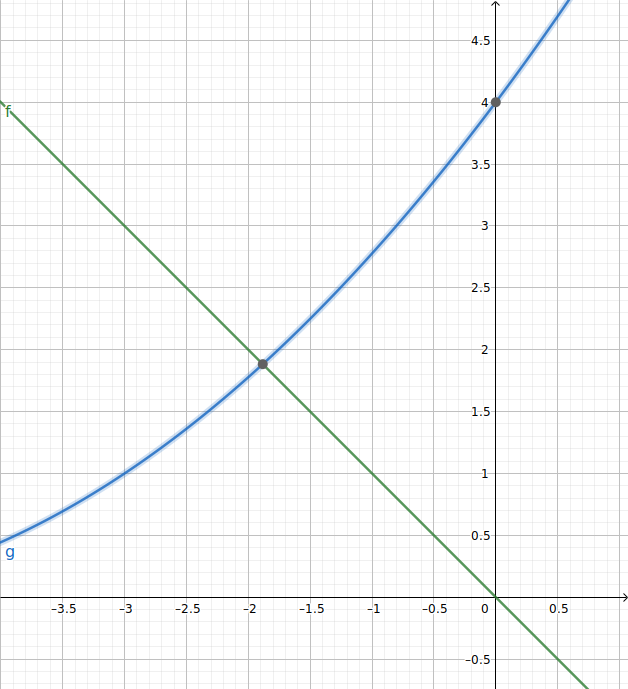
\includegraphics[width=0.7\linewidth]{images/geogebra.pdf}}
\caption{Intersección entre curvas. Eje horizonal medido en $V$. Eje vertical medido en $mA$}
\label{4.6}
\end{figure}





      %\cite{fis}

\bigskip
           \newpage
                   \printbibliography 
\bigskip

\end{document}
